\section*{HOJA DE CONTROL}
%\section*{CONTROL SHEET}
\thispagestyle{empty}

     \vspace{1cm}

\begin{table}[!htb]
    \centering
    \begin{tabular}{|p{3cm}|p{8cm}|}
        \hline
         \cellcolor{gray30}  Asignatura	& \asignatura\\ 
%      \cellcolor{gray30}  Subject	& \asignatura\\   
   
         \hline
         \cellcolor{gray30}  Entregable & \tipoDoc\\  
%        \cellcolor{gray30}  Deliverable & \tipoDoc\\           
        \hline
         \cellcolor{gray30}  Autor	& \equipo  \\
%      \cellcolor{gray30}  Author	& \equipo  \\   
        \hline
         \cellcolor{gray30}  Versión	& -num version\\   
%         \cellcolor{gray30}  Version	& -num version\\   
        \hline
         \cellcolor{gray30}  Fecha	& \today \\  
%      \cellcolor{gray30}  Date	& \today \\            
        \hline
    \end{tabular}
  \end{table}



\textbf{ REGISTRO DE CAMBIOS}
%\textbf{ CHANGES LOG}

\begin{table}[!htb]
    \centering
    \begin{tabular}{|p{7ex}|p{20ex}|p{25ex}|p{8ex}|}
        \hline
         \rowcolor{gray30}  Versión	& Causa del cambio& Responsable & Fecha\\ 
%        \rowcolor{gray30}  Version	& Change cause& Who& Date\\   
        \hline
        0100 &  Versión inicial    & $<Nombre>$   	&  \\   
        \hline
          &     &    	&  \\     
        \hline
    \end{tabular}
\end{table}


	\textbf{LISTA DE DISTRIBUCIÓN}
%     \textbf{DISTRIBUTION LIST}


\begin{table}[!htb]
    \centering
    \begin{tabular}{|p{50ex}|}
        \hline
         \rowcolor{gray30} 	Nombre y Apellidos\\   
%        \rowcolor{gray30} 	Name and surname\\            
        \hline
         Isabel María del Águila Cano\\
        \hline
         \primerAl\\     
        \hline
        \segunAl\\
        \hline
        \tercerAl\\
       \hline
        \end{tabular}
\end{table}

\cleardoublepage

%\tableofcontents
%\listoffigures
%\listoftables

\newcommand{\fig}{SRS/Figuras}




% ********************************************************************
% Re-usable information
%********************************************************************

\renewcommand {\tipoDoc} {Especificación de los requisitos del software}
%\newcommand {\tipoDoc} {Software Requirements Specification}
\newcommand {\miProyecto} {Nombre e Id del proyecto}
%\newcommand {\miProyecto} {project name and Id}


%\hyphenation{}



%%%% Definición de las cabeceras

%\usepackage{fancyhdr}

\pagestyle{fancy}
\fancyhf{}

\fancyhead[LE]{ \textbf{\thepage} \ \ \ Equipo: \equipo   }
%\fancyhead[LE]{ \textbf{\thepage} \ \ \ Team: \equipo   }
\fancyhead[RO]{ Equipo: \equipo  \ \ \ \textbf{\thepage}}
%\fancyhead[RO]{ Team: \equipo  \ \ \ \textbf{\thepage}}
\fancyhead[LO]{
\includegraphics[width=0.15\textwidth]{Cabecera/imagenes/inre.png} \miProyecto  }
\fancyhead[RE]{\miProyecto 
\includegraphics[width=0.15\textwidth]{Cabecera/imagenes/inre.png}   }

\renewcommand{\sectionmark}[1]{\markright{\textbf{\thesection. #1}}}

\setlength{\headheight}{2\headheight}




\newfloat{Artefacto}{tbp}{loa}[section]     %% Float de artefacto requisito 
   \setlength{\parskip}{3mm}     % !
  \setlength{\parindent}{3mm}   % !
  \frenchspacing
  \sloppy
  
\newfloat{Artifact}{tbp}{loa}[section]    
   \setlength{\parskip}{3mm}     % !
  \setlength{\parindent}{3mm}   % !
  \frenchspacing
  \sloppy
  


\newfloat{RF}{tbp}{loa}[section]     %% Float de requisito funcional
   \setlength{\parskip}{3mm}     % !
  \setlength{\parindent}{3mm}   % !
  \frenchspacing
  \sloppy

\newfloat{R}{tbp}{loa}[section]     %% Float de requisito información
   \setlength{\parskip}{3mm}     % !
  \setlength{\parindent}{3mm}   % !
  \frenchspacing
  \sloppy

\newfloat{RNF}{tbp}{loa}[section]     %% Float de requisito no funcional
   \setlength{\parskip}{3mm}     % !
  \setlength{\parindent}{3mm}   % !
  \frenchspacing
  \sloppy

\newfloat{ACT}{tbp}{loa}[section]     %% Float de requisito no funcional
   \setlength{\parskip}{3mm}     % !
  \setlength{\parindent}{3mm}   % !
  \frenchspacing
  \sloppy
  
  \newfloat{PRO}{tbp}{loa}[section]     %% Float de requisito no funcional
   \setlength{\parskip}{3mm}     % !
  \setlength{\parindent}{3mm}   % !
  \frenchspacing
  \sloppy
 
   \newfloat{OBJ}{tbp}{loa}[section]     %% Float de requisito no funcional
   \setlength{\parskip}{3mm}     % !
  \setlength{\parindent}{3mm}   % !
  \frenchspacing
  \sloppy
     %definición de artefactos y similares

%TEXTO PROPIAMENTE DICHO

\begin{titlepage}
 

%\newlength{\centeroffset}
%\setlength{\centeroffset}{-0.5\oddsidemargin}
%\addtolength{\centeroffset}{0.5\evensidemargin}
%\thispagestyle{empty}

\noindent\hspace*{\centeroffset}\begin{minipage}{\textwidth}

\centering

\includegraphics[width=0.8\textwidth]{\folder/Portada/imagenes/logo_ual.jpg}\\[0.8cm]

\textsc{ \Huge \miProyecto \\[0.7cm]}

{\Huge\bfseries \tipoDoc \\ }
\noindent\rule[-1ex]{\textwidth}{3pt}\\[3ex]

\end{minipage}

\vspace{2.3cm}
\noindent\hspace*{\centeroffset}\begin{minipage}{\textwidth}
\centering


\includegraphics[width=0.5\textwidth]{\folder/Portada/imagenes/inre.png}\\[0.1cm]

\textsc{---}\\
Almería, \today \\[1cm]

\textbf{Equipo:} {\equipo}\\[0.2cm]
%\textbf{Team:} {\equipo}\\[0.2cm]
\textbf{Miembros:}\\ {\primerAl\\ \segunAl \\ \tercerAl}\\[1cm]
%\textbf{Members:}\\ {\primerAl\\ \segunAl \\ \tercerAl}\\[1cm]


\end{minipage}

\end{titlepage}




\section*{HOJA DE CONTROL}
%\section*{CONTROL SHEET}
\thispagestyle{empty}

     \vspace{1cm}

\begin{table}[!htb]
    \centering
    \begin{tabular}{|p{3cm}|p{8cm}|}
        \hline
         \cellcolor{gray30}  Asignatura	& \asignatura\\ 
%      \cellcolor{gray30}  Subject	& \asignatura\\   
   
         \hline
         \cellcolor{gray30}  Entregable & \tipoDoc\\  
%        \cellcolor{gray30}  Deliverable & \tipoDoc\\           
        \hline
         \cellcolor{gray30}  Autor	& \equipo  \\
%      \cellcolor{gray30}  Author	& \equipo  \\   
        \hline
         \cellcolor{gray30}  Versión	& -num version\\   
%         \cellcolor{gray30}  Version	& -num version\\   
        \hline
         \cellcolor{gray30}  Fecha	& \today \\  
%      \cellcolor{gray30}  Date	& \today \\            
        \hline
    \end{tabular}
  \end{table}



\textbf{ REGISTRO DE CAMBIOS}
%\textbf{ CHANGES LOG}

\begin{table}[!htb]
    \centering
    \begin{tabular}{|p{7ex}|p{20ex}|p{25ex}|p{8ex}|}
        \hline
         \rowcolor{gray30}  Versión	& Causa del cambio& Responsable & Fecha\\ 
%        \rowcolor{gray30}  Version	& Change cause& Who& Date\\   
        \hline
        0100 &  Versión inicial    & $<Nombre>$   	&  \\   
        \hline
          &     &    	&  \\     
        \hline
    \end{tabular}
\end{table}


	\textbf{LISTA DE DISTRIBUCIÓN}
%     \textbf{DISTRIBUTION LIST}


\begin{table}[!htb]
    \centering
    \begin{tabular}{|p{50ex}|}
        \hline
         \rowcolor{gray30} 	Nombre y Apellidos\\   
%        \rowcolor{gray30} 	Name and surname\\            
        \hline
         Isabel María del Águila Cano\\
        \hline
         \primerAl\\     
        \hline
        \segunAl\\
        \hline
        \tercerAl\\
       \hline
        \end{tabular}
\end{table}

\cleardoublepage

%\tableofcontents
%\listoffigures
%\listoftables


\clearpage

\thispagestyle{fancy}
\section{Introducción}
%\section{Introduction}
 
\begin{textoazul}
Esta sección obligatoria debe contener información relativa al dominio del problema que permita comprender los conceptos básicos del mismo al lector del documento. Se divide en las secciones que se describen a continuación.
La información de esta sección puede que ya se encuentre total o parcialmente en documentación previa como el Pliego de Prescripciones Técnicas, la Oferta seleccionada o el Estudio de Viabilidad del Sistema, en cuyo se podrá reutilizar y se hará referencia a dichos documentos como fuente de la misma.

%This mandatory section must contain problem domain related information for understanding the basics of concepts. It is divided into the sections described below.
%The information may already be full or pArtefactoially found in previous documentation, as the technical specifications or initial preprojects, in this case, can be reused.
\end{textoazul}

 \subsection {Alcance} 
 % \subsection {Scope}

\begin{textoazul}
Esta sección debe describir a qué elementos organizativos de la empresa afecta el desarrollo del nuevo sistema
% You must include the issues related to the business organization that are relevant for the new system 
 \end{textoazul}
 
 \subsection {Objetivos}
% \subsection {Goals}
  
\begin{textoazul}
Esta sección debe describir los principales objetivos que se esperan alcanzar cuando el sistema a desarrollar esté en producción.

%the main goals for the new system have to be described
 \end{textoazul}
 


\section{Información del dominio del problema}

%\section{Problem domain information}
  l
\begin{textoazul}
 
 Esta sección obligatoria debe contener información relativa al dominio del problema que permita comprender los \textbf{conceptos básicos} del mismo al lector del documento. Se divide en las secciones que se describen a continuación.
 
 %this mandatory section shoudl contains problem domain information 
\end{textoazul}
 
\subsection{Introducción al Dominio del Problema}

 \begin{textoazul}
 Se trata de dar una visión general del conjunto de conceptos que se manejan en la organización para la que se va a desarrollar el sistema software. Pueden incluirse diagramas u otro elemento multimedia si se considera oportuno para facilitar su comprensión.
 
 % Overview of the concepts managed by the organization. You can include diagrams or any other description method
 \end{textoazul}
 
\subsection{Glosario de Términos}
%\subsection{Glossary}

 \begin{textoazul}
 Esta sección debe contener una lista ordenada alfabéticamente de los principales términos, acrónimos y abreviaturas específicos del dominio del problema, especialmente de los que se considere que su significado deba ser aclarado. Cada término, acrónimo o abreviatura deberá acompañarse de su definición y se podrá adjuntar material multimedia que facilite su comprensión como fotografías, documentos escaneados, diagramas o incluso vídeo o sonido en el caso de que el formato de la ERS lo permita

% This section should contain an alphabetical list of key terms, acronyms and abbreviations specific problem domain, especially those deemed that its meaning should be clarified. Each term, acronym or abbreviation must be accompanied by its definition and multimedia material may be attached to facilitate its understanding as photographs, scanned documents, diagrams or even video or sound in case the SRS format permits
\end{textoazul}

\section{Descripción de la situación actual [optional]} 
%\section{Current situation}

\begin{textoazul}
  Esta sección opcional debe contener información sobre la situación actual de la organización para la que se va a desarrollar el sistema software. En concreto, debe contener información sobre los pros y contras de la situación actual, sobre los modelos de proceso de negocio actuales y sobre el entorno tecnológico actual de la organización, incluyendo la arquitectura orientada a servicios actual si existiera. Se divide en las secciones que se describen a continuación.

Esta sección podrá omitirse total o parcialmente si se considera que la situación actual es suficientemente conocida por todos los pArtefactoicipantes en el proyecto.

%This section is totally or pArtefactoially optional and it should contain the current business state. Specifically do's and don'ts, including a description of the main business processes that could be modified by the new system.

\end{textoazul}



\subsection{Modelos de Procesos de Negocio Actuales}
%\subsection{Current Business process models}

\begin{textoazul}
Esta sección debe contener información sobre los modelos de procesos de negocio actuales, que suelen ser la base de los modelos de procesos de negocio a implantar.

%current business process models 

  \end{textoazul}
 

\subsubsection{Descripción de los Actores de Negocio Actuales}
%\subsubsection{Current business actors}

\begin{textoazul}
Esta sección debe contener información sobre los actores de negocio (organizaciones, roles o responsabilidades) de los modelos de procesos de negocio actuales especificados mediante las plantillas para actores del negocio actual. Lo indicado con corchetes es adicional. Copiar cuantas veces sea necesario

 \end{textoazul}

 \begin{Artefacto}[H]
    \centering
    \begin{tabular}{|p{3cm}|p{10cm}|}
        \hline
         \cellcolor{gray30}  NEG-ACT 999	&  $<nombre descriptivo>$\\ 
%      \cellcolor{gray30}  BUS-ACT 999	& <descriptive name>\\   
        \hline
         \cellcolor{gray30}  [Versión]	&  $<num version(fecha de version>$)\\   
%      \cellcolor{gray30}  [Version]	&   $<num version(date>$)\\   
         \hline
         \cellcolor{gray30}  [Dependencias] &  	\begin{itemize} \item $<procesos de negocio actuales en los que participa>$
\item	... \end{itemize}\\  
%                 \cellcolor{gray30}  [Dependencies] &  	\begin{itemize} \item $<business processes this actor is involved in>$
%\item	... \end{itemize}\\            
        \hline
         \cellcolor{gray30} Descripción	& Este actor de negocio actual representa a $<descripcion$ $de la organizacion, rol  o responsabilidad  a la que$ $representa  el actor de negocio actual>$  \\
%      \cellcolor{gray30}   Description	& descrip\\   
        \hline
         \cellcolor{gray30}  Comentarios	&$<comentarios adicionales sobre el actor  de $ $negocio  actual>$\\   
%         \cellcolor{gray30} Comments	&$<$additional comments$>$
        \hline
  
    \end{tabular}
\caption{NEG-ACT 999	$<nombre descriptivo>$ }
%\caption{BUS-ACT 999	$<descriptive name >$ }
  \end{Artefacto}

 


\subsubsection{	Descripción de Procesos de Negocio Actuales}

%\subsubsection{Description of the current business processes}


 \begin{Artefacto}[H]
    \centering
    \begin{tabular}{|p{3cm}|p{10cm}|}
        \hline
         \cellcolor{gray30}  NEG-PRO 999	&  $<nombre descriptivo>$\\ 
%      \cellcolor{gray30}  BUS-PRO 999	& <descriptive name>\\   
        \hline
         \cellcolor{gray30}  [Versión]	&  $<n version>(<fecha de version>$)\\   
%      \cellcolor{gray30}  [Version]	&   $<n version>$($<date>$)\\   
         \hline
         \cellcolor{gray30}  [Dependencias] &  	\begin{itemize} \item $<$procesos de negocio actuales en los que participa$>$
\item	... \end{itemize}\\  
%                 \cellcolor{gray30}  [Dependencies] &  	\begin{itemize} \item $<business processes this actor is involved in>$
%\item	... \end{itemize}\\            
        \hline
        \cellcolor{gray30} Descripción	& Este proceso $<descripcion>$ \\
%      \cellcolor{gray30}   Description	& descrip\\   
        \hline
         \cellcolor{gray30}Importancia	& $<importancia del proceso de negocio para el cliente>$  \\
%      \cellcolor{gray30}   Importance 	& descrip\\   
        \hline
           \cellcolor{gray30}  [Actores] &  	\begin{itemize} \item $<actor que participa en el proceso de negocio actual>$
\item	... \end{itemize}\\  
%                 \cellcolor{gray30}  [Actors] &  	\begin{itemize} \item $<actor involved in the business process>$
%\item	... \end{itemize}\\
         \hline
         \cellcolor{gray30}  Comentarios	&$<comentarios adicionales sobre actor de negocio actual>$\\   
%         \cellcolor{gray30} Comments	&$<additional comments>$
        \hline
  
    \end{tabular}
\caption{NEG-PRO 999	$<nombre descriptivo>$ }
%\caption{BUS-PRO 999	$<descriptive name >$ }
  \end{Artefacto}






\subsection{	Entorno Tecnológico Actual}
%\subsection{ Current Technological environment}

 
\subsubsection{	Descripción del Entorno de Hardware Actual}
%\subsubsection{	Current Hardware }
 
\subsubsection{	Descripción del Entorno de Software Actual}
%\subsubsection{	Current Software }

 

\section{Necesidades del negocio}

\begin{textoazul}
Esta sección obligatoria debe contener información sobre los objetivos de negocio de clientes y usuarios, incluyendo los modelos de procesos de negocio a implantar. Esta sección se divide en las secciones que se describen a continuación.

La información de esta sección puede que ya se encuentre total o parcialmente en documentación previa como el Pliego de Prescripciones Técnicas, la Oferta seleccionada o el Estudio de Viabilidad del Sistema, en cuyo se podrá reutilizar y se hará referencia a dichos documentos como fuente de la misma.
\end{textoazul}
 
\subsection{Objetivos de Negocio}
\begin{textoazul}
Esta sección debe contener los objetivos de negocio que se esperan alcanzar cuando el sistema software a desarrollar esté en producción, especificados mediante las  plantillas de objetivos de negocio que se muestran a continuación. En el caso de que se considere necesario, los objetivos de negocio se pueden descomponer jerárquicamente para facilitar su comprensión y representar dicha jerarquía de forma gráfica.
 \end{textoazul}




 \begin{Artefacto}[H]
    \centering
    \begin{tabular}{|p{3cm}|p{10cm}|}
        \hline
         \cellcolor{gray30}  NEG-OBJ 999	&  $<$nombre descriptivo$>$\\ 
%      \cellcolor{gray30}  BUS-OBJ 999	& <descriptive name>\\   
        \hline
         \cellcolor{gray30}  [Versión]	&  $<$nº versión$>$($<$fecha de versión$>$)\\   
%      \cellcolor{gray30}  [Version]	&   $<$nº version$>$($<$date$>$)\\   
         \hline
         \cellcolor{gray30}  [Dependencias] &  	\begin{itemize} \item $<procesos de negocio actuales en los que participa>$
\item	... \end{itemize}\\  
%                 \cellcolor{gray30}  [Dependencies] &  	\begin{itemize} \item $<business processes this actor is involved in>$
%\item	... \end{itemize}\\            
        \hline
        \cellcolor{gray30} Descripción	& Este objetivo representa  \\
%      \cellcolor{gray30}   Description	& descrip\\   
        \hline
                 \cellcolor{gray30}  Subobjetivos &  	\begin{itemize} \item $<objetivos del negocio hijos>$
\item	... \end{itemize}\\  
%                 \cellcolor{gray30}  [Subobjectives] &  	\begin{itemize} \item<subobjetives >$
%\item	... \end{itemize}\\            
        \hline
         \cellcolor{gray30}Importancia	& $<importancia del proceso de negocio para el cliente>$  \\
%      \cellcolor{gray30}   Importance 	& descrip\\   
        \hline
          \cellcolor{gray30}  [Prioridad] &  	$<prioridad del objetivo de negocio para la direccion$ $ del proyecto>$\\
%                 \cellcolor{gray30}  [Priority] &   	\\
         \hline
         \cellcolor{gray30}  Comentarios	&$<comentarios adicionales sobre el actor de negocio actual>$\\   
%         \cellcolor{gray30} Comments	&$<additional comments>$
        \hline
  
    \end{tabular}
\caption{NEG-OBJ 999	$<nombre descriptivo>$ }
%\caption{BUS-OBJ 999	$<descriptive name>$ }
  \end{Artefacto}


\subsection{Modelos de Procesos de Negocio a Implantar} 

\begin{textoazul}
Esta sección opcional, debe contener los modelos de procesos de negocio a implantar, que normalmente son los modelos de procesos de negocio actuales con ciertas mejoras. Si las diferencias con los modelos de procesos actuales son pequeñas, se puede optar por describir únicamente dichas diferencias siempre que se hayan incluido los modelos de procesos actuales en la sección 3.2.
\end{textoazul}
 
 
 
 \begin{Artefacto}[H]
 \centering
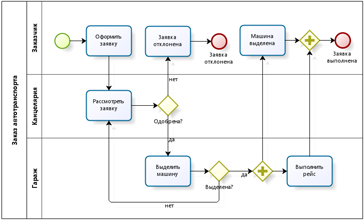
\includegraphics[width=0.8\textwidth]{\fig/BPMN.png}
 \caption{NEG-MOD 999	$<nombre descriptivo>$}
 \end{Artefacto}
 
\subsubsection{Descripción de los Actores de Negocio a Implantar}

 
 \begin{Artefacto}[H]
    \centering
    \begin{tabular}{|p{3cm}|p{10cm}|}
        \hline
         \cellcolor{gray30}  NEG-ACT 999	&  $<nombre descriptivo>$\\ 
%      \cellcolor{gray30}  BUS-ACt 999	& <descriptive name>\\   
        \hline
         \cellcolor{gray30}  [Versión]	&  $<$nº versión$>$($<$fecha de versión$>$)\\   
%      \cellcolor{gray30}  [Version]	&   $<$nº version$>$($<$date$>$)\\   
         \hline
         \cellcolor{gray30}  [Dependencias] &  	\begin{itemize} \item $<procesos de negocio  en los que participara>$
\item	... \end{itemize}\\  
%                 \cellcolor{gray30}  [Dependencies] &  	\begin{itemize} \item $<business processes this actor will be involved in>$
%\item	... \end{itemize}\\            
        \hline
         \cellcolor{gray30} Descripción	& Este actor de negocio  representa a $<descripcion de la organizacion, rol  o responsabilidad$ $  a la que representa  el actor de negocio a implantar>$  \\
%      \cellcolor{gray30}   Description	& descrip\\   
        \hline
         \cellcolor{gray30}  Comentarios	&$<comentarios adicionales actor de negocio  a implantar>$\\   
%         \cellcolor{gray30} Comments	&$<additional comments>$
        \hline
  
    \end{tabular}
\caption{NEG-ACT 999	$<nombre descriptivo>$ }
%\caption{BUS-ACT 999	$<descriptive name>$ }
  \end{Artefacto}




\subsubsection{Descripción de Procesos de Negocio a Implantar}
 

 \begin{Artefacto}[H]
    \centering
    \begin{tabular}{|p{3cm}|p{10cm}|}
        \hline
         \cellcolor{gray30}  NEG-PRO 999	&  $<nombre descriptivo>$\\ 
%      \cellcolor{gray30}  BUS-PRO 999	& <descriptive name>\\   
        \hline
         \cellcolor{gray30}  [Versión]	&  $<$nº versión$>$($<$fecha de versión$>$)\\   
%      \cellcolor{gray30}  [Version]	&   $<$nº version$>$($<$date$>$)\\   
         \hline
         \cellcolor{gray30}  [Dependencias] &  	\begin{itemize} \item $<procesos de negocio a implantar $ $en los que participa>$
\item	... \end{itemize}\\  
%                 \cellcolor{gray30}  [Dependencies] &  	\begin{itemize} \item $<$business processes this actor is involved in$>$
%\item	... \end{itemize}\\            
        \hline
        \cellcolor{gray30} Descripción	& Este procesos  \\
%      \cellcolor{gray30}   Description	& descrip\\   
        \hline
         \cellcolor{gray30}[Importancia]	& $<importancia del proceso de negocio para el cliente>$  \\
%      \cellcolor{gray30}   Importance 	& descrip\\   
        \hline
           \cellcolor{gray30}  [Actores] &  	\begin{itemize} \item $<actor que participa en el proceso $ $de negocio implantar>$
\item	... \end{itemize}\\  
%                 \cellcolor{gray30}  [Actors] &  	\begin{itemize} \item $<$actor involved in the business process$>$
%\item	... \end{itemize}\\
         \hline
         \cellcolor{gray30}  Comentarios	&$<comentarios adicionales del actor$ $ de negocio a implantar>$\\   
%         \cellcolor{gray30} Comments	&$<$additional comments$>$
        \hline
  
    \end{tabular}
\caption{NEG-PRO 999	$<$nombre descriptivo$>$ }
%\caption{BUS-PRO 999	$<$descriptive name $>$ }
  \end{Artefacto}

\section{Descripcion de los subsistemas del sistema a desarrollar} 
\begin{textoazul}
Incluir si es necesario la descomposición del sistema en subsistemas. Se incluirá un diagrama de bloques u organigramapor claridad

Esta sección podrá omitirse si el sistema software a desarrollar es lo suficientemente sencillo como para no ser dividido en subsistemas.
\end{textoazul}


 \begin{Artefacto}[H]
 \centering
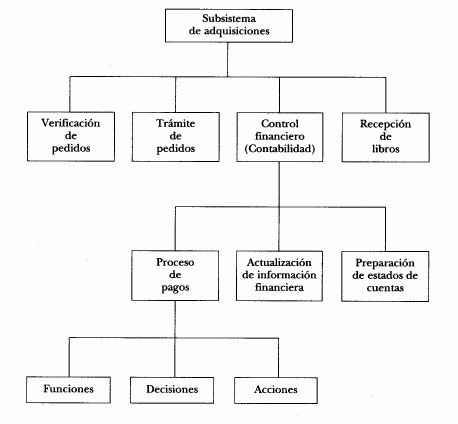
\includegraphics[width=0.8\textwidth]{\fig/organi.jpg}
 \caption{SUB 999	$<nombre descriptivo>$}
 \end{Artefacto}


 \begin{Artefacto}[H]
    \centering
    \begin{tabular}{|p{3cm}|p{10cm}|}
        \hline
         \cellcolor{gray30}  SUB-PRO 999	&  $<nombre descriptivo>$\\ 
%      \cellcolor{gray30}  SUB-PRO 999	& <descriptive name>\\   
        \hline
         \cellcolor{gray30}  [Versión]	&  $<$nº versión$>$($<$fecha de versión$>$)\\   
%      \cellcolor{gray30}  [Version]	&   $<$nº version$>$($<$date$>$)\\   
         \hline
         \cellcolor{gray30}  [Dependencias] &  	\begin{itemize} \item $<objetivos de negocio que comprende>$
\item	$<proceso de negocio con que se relaciona>$ \end{itemize}\\  
%                 \cellcolor{gray30}  [Dependencies] &  	\begin{itemize} \item $<$business processes this actor is involved in$>$
%\item	... \end{itemize}\\            
        \hline
        \cellcolor{gray30} Descripción	& Este subsistema representa a $<descripcion >$  \\
%      \cellcolor{gray30}   Description	& descrip\\   
        \hline
         \cellcolor{gray30}[Importancia]	& $<importancia del proceso de negocio para el cliente>$  \\
%      \cellcolor{gray30}   [Importance] 	& descrip\\   
        \hline
         \cellcolor{gray30}  [Prioridad] &  	$<prioridad para la direccion del proyecto>$\\
%                 \cellcolor{gray30}  [Priority] &   	\\  
         \hline
         \cellcolor{gray30}  Comentarios	&$<comentarios adicionales >$\\   
%         \cellcolor{gray30} Comments	&$<$additional comments$>$
        \hline
  
    \end{tabular}
\caption{SUB-999	$<nombre descriptivo>$ }
%\caption{SUB-999	$<descriptive name>$ }
  \end{Artefacto}




\section{Requisitos del sistema a desarrollar}


 \begin{figure}[H]
 \centering
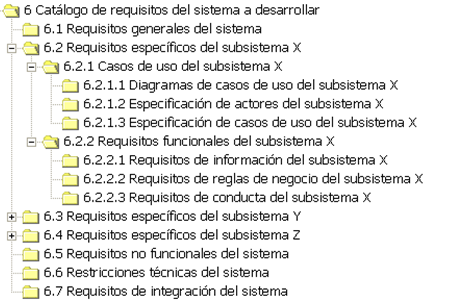
\includegraphics[width=0.8\textwidth]{\fig/indice.png}
 \caption{Ejemplo del índice}
 \end{figure}
 

\subsection{Requisitos Generales del Sistema [Opcional]}


 \begin{textoazul}
 Esta sección debe contener la especificación de los requisitos generales del sistema, también denominados características del sistema (system features) u objetivos del sistema, especificados mediante las  plantillas para requisitos generales que se muestran a continuación.
 

Los requisitos generales puede que ya se encuentren alineados con los objetivos del negocio. En el caso de que se considere necesario, los requisitos generales se podrán descomponer jerárquicamente para facilitar su comprensión.

\end{textoazul}

 \begin{Artefacto}[H]
    \centering
    \begin{tabular}{|p{3cm}|p{10cm}|}
        \hline
         \cellcolor{gray30}  REQ-GEN 999	&  $<nombre descriptivo>$\\ 
%      \cellcolor{gray30}  REQ-GEN 999	& <descriptive name>\\   
        \hline
         \cellcolor{gray30}  [Versión]	&  $<num version(fecha de version>$)\\   
%      \cellcolor{gray30}  [Version]	&   $<num version(date>$)\\   
         \hline
         \cellcolor{gray30}  [Dependencias] &  	\begin{itemize} 	\item $<requisito general padre, si lo tiene (padre)>$
\item $<otros requisitos generales de los que dependa>$
\item	... \end{itemize}\\  
%                 \cellcolor{gray30}  [Dependencies] &  	\begin{itemize} \item requirement
%\item	... \end{itemize}\\            
        \hline
         \cellcolor{gray30} Descripción	& $<descripcion>$  \\
%      \cellcolor{gray30}   Description	& \\   
          \hline
         \cellcolor{gray30}  Requisitos hijos&  	\begin{itemize} 	\item  
\item 
\item	... \end{itemize}\\  
%                 \cellcolor{gray30}  [Dependencies] &  	\begin{itemize} \item requirement
%\item	... \end{itemize}\\            
        \hline          
           \cellcolor{gray30}[Importancia]	& $<importancia para el cliente>$  \\
%      \cellcolor{gray30}   [Importance] 	& descrip\\   
         \hline
         \cellcolor{gray30}  [Prioridad] &  	$<prioridad para la direccion del proyecto>$\\
%                 \cellcolor{gray30}  [Priority] &   	\\  
         \hline
         \cellcolor{gray30}  [Estado]	&$<estado del requisito segun el ciclo de vida $ $ adoptado por el proyecto>$\\   
%         \cellcolor{gray30} State	&$<state according the lifecicle>$
        \hline       
         \cellcolor{gray30}  Comentarios	&$<comentarios adicionales $\\   
%         \cellcolor{gray30} Comments	&$<additional comments>$
        \hline
  
    \end{tabular}
\caption{REQ-GEN 999	$<nombre descriptivo>$ }
%\caption{REQ-GEN 999	$<descriptive name >$ }
  \end{Artefacto}



\subsection{Casos de uso del Sistema}
\begin{textoazul}
 Esta sección debe contener la especificación de los casos de uso del sistema, denominados escenarios operacionales en terminología CMMI-DEV, incluyendo los correspondientes diagramas, la especificación de los actores y la especificación de los propios casos de uso. Los casos de uso deben describir cómo se utilizará el sistema a desarrollar por sus futuros usuarios para realizar sus procesos de negocio
\end{textoazul} 
 
\subsubsection{Diagramas de Casos de Uso del Sistema}

 
  \begin{figure}[H]
\centering
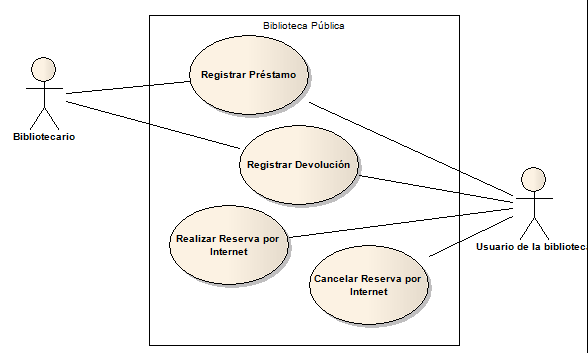
\includegraphics[width=0.8\textwidth]{\fig/casos.png}
\caption{Ejemplo del diagrama de casos de uso}
\end{figure}



\subsubsection{Especificación de Actores del Sistema}
<Introduzca contenido, cumplimente tabla y borre cuadro>

  \begin{Artefacto}[H]
    \centering
    \begin{tabular}{|p{3cm}|p{10cm}|}
        \hline
         \cellcolor{gray30}  CDU-ACT 999	&  $<nombre descriptivo>$\\ 
%      \cellcolor{gray30}  CDU-ACT 999	& <descriptive name>\\   
        \hline
         \cellcolor{gray30}  [Versión]	&  $<num version(fecha de version>$)\\   
%      \cellcolor{gray30}  [Version]	&   $<nº version>$($<date>$)\\   
         \hline
         \cellcolor{gray30}  [Dependencias] &  	\begin{itemize} \item $<actores del negocio relacionados>$\item	... \end{itemize}\\  

%                 \cellcolor{gray30}  [Dependencies] &  	\begin{itemize} \item $<related business actors>$
%\item	... \end{itemize}\\            
        \hline
         \cellcolor{gray30} Descripción	& $<descripcion del rol que representa el actor en$ $ los casos de uso del sistema >$ \\
%      \cellcolor{gray30}   Description	& descrip\\   
        \hline
         \cellcolor{gray30}  Comentarios	&$<comentarios adicionales sobre el actor de negocio  a$ $ implantar>$\\   
%         \cellcolor{gray30} Comments	&$<additional comments>$
        \hline
  
    \end{tabular}
\caption{CDU-ACT 999	$<nombre descriptivo>$ }
%\caption{CDU-ACT 999	$<descriptive name >$ }
  \end{Artefacto}



\subsubsection{Especificación de Casos de Uso del Sistema}


 


\begin{Artefacto}[H]
    \centering
    \begin{tabular}{|p{3cm}|p{10cm}|}
        \hline
         \cellcolor{gray30}  CDU-999	&  $<nombre descriptivo>$\\ 
%      \cellcolor{gray30}  REQ-GEN 999	& <descriptive name>\\   
        \hline
         \cellcolor{gray30}  [Versión]	&  $<num version(fecha de version>$)\\   
%      \cellcolor{gray30}  [Version]	&   $<num version>$($<date>$)\\   
         \hline
         \cellcolor{gray30}  [Dependencias] &  	\begin{itemize} 	\item $<requisitos generales de los que depende>$
\item $<otros requisitos generales de los que dependa>$
\item	... \end{itemize}\\  
%                 \cellcolor{gray30}  [Dependencies] &  	\begin{itemize} \item requirement
%\item	... \end{itemize}\\            
        \hline
         \cellcolor{gray30} Descripción	&El sistema deberá comportarse tal como se indica en la siguiente especificación del caso de uso\\
%      \cellcolor{gray30}   Description	& descrip\\   
\hline
          
         \cellcolor{gray30}  Secuencia normal&  	
         \begin{enumerate} 	
             \item	{El actor $<$actor del sistema$>$, El sistema}<acción/es realizada/s por el actor del sistema>
			\item	Se realiza el $<$caso de uso del sistema$>$
			\item	Si <condición>,
            ...	...
            \begin{enumerate}
		       \item El caso de uso termina con éxito,Se cancela el caso de uso
               \item
       
        	\end{enumerate}
	...	...\item paso 
													
       \item	... \end{enumerate}\\  

\hline          
  \cellcolor{gray30} Postcondición	& postcondición del caso de uso del sistema \\
  \hline
 \cellcolor{gray30}  Excepciones&
 \begin{itemize} 	        
			\item	$<$PASO m$>$	Si $<$condición de excepción$>$
            \begin {enumerate}
            \item 	{El caso de uso continua,Se cancela el caso de uso}
            \item
            \end{enumerate}
            \item	$<$PASO n$>$: 
 \end{itemize}\\ 
\hline
        \hline          
           \cellcolor{gray30}[Importancia]	& $<importancia del requisito para el cliente>$  \\
%      \cellcolor{gray30}   Importance 	& descrip\\   
         \hline
         \cellcolor{gray30}  [Prioridad] &  	$<prioridad del requisito para la direccion del proyecto>$\\
%                 \cellcolor{gray30}  [Priority] &   	\\  
         \hline
         \cellcolor{gray30}  Estado	&$<estado  segun el ciclo de vida adoptado por el proyecto>>$\\   
%         \cellcolor{gray30} State	&$<state according the lifecicle>$
        \hline       
         \cellcolor{gray30}  Comentarios	& $<comentarios adicionales>$ \\   
%         \cellcolor{gray30} Comments	&$<additional comments>$
        \hline
  
    \end{tabular}
\caption{CDU 999	$<nombre descriptivo>$ }
%\caption{CDU 999	$<descriptive name >$ }
  \end{Artefacto}











\subsection{Requisitos Funcionales del Sistema}

\begin{textoazul}
Esta sección debe contener los requisitos funcionales del sistema que se hayan identificado a partir de los requisitos generales, de los casos de uso del sistema o de otras fuentes. Se divide en las secciones que se describen a continuación.
\end{textoazul}
  

            
\subsubsection{Requisitos de Información del Sistema}
<Introduzca contenido, cumplimente tabla y borre cuadro>
 
 
   \begin{figure}[H]
 \centering
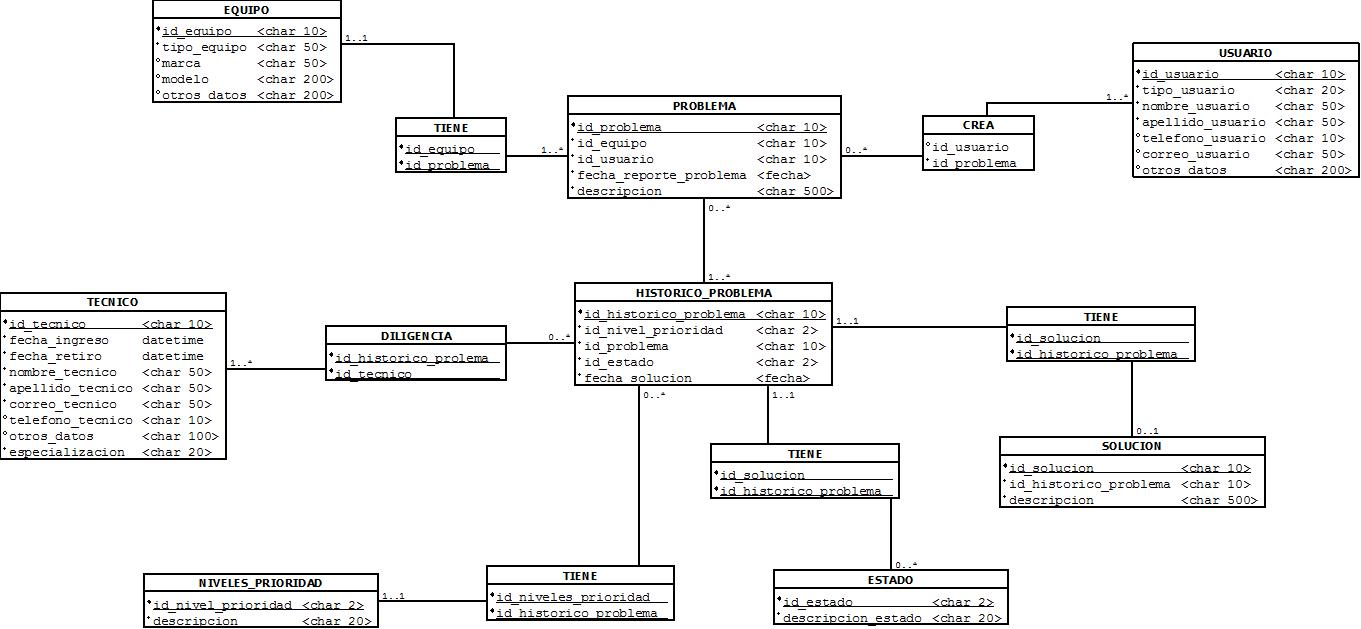
\includegraphics[width=0.8\textwidth]{\fig/datos.jpg}
 \caption{Ejemplo de modelo de datos}
 \end{figure}
 



\begin{Artefacto}[H]
    \centering
    \begin{tabular}{|p{3cm}|p{10cm}|}
        \hline
         \cellcolor{gray30}  REQ-GEN 999	&  $<nombre descriptivo>$\\ 
%      \cellcolor{gray30}  REQ-GEN 999	& <descriptive name>\\   
        \hline
         \cellcolor{gray30}  [Versión]	&  $<num version(fecha de version>$)\\   
%      \cellcolor{gray30}  [Version]	&   $<num version>$($<date>$)\\   
         \hline
         \cellcolor{gray30}  [Dependencias] &  	\begin{itemize} 	\item $<requisitos generales de los que depende>$
\item $<otros requisitos generales de los que dependa>$
\item	... \end{itemize}\\  
%                 \cellcolor{gray30}  [Dependencies] &  	\begin{itemize} \item requirement
%\item	... \end{itemize}\\            
        \hline
         \cellcolor{gray30} Descripción	&El sistema deberá almacenar la información correspondiente a <concepto relevante>. En concreto:\\
%      \cellcolor{gray30}   Description	& descrip\\   
          \hline
         \cellcolor{gray30}  Datos específicos&  	\begin{itemize} 	\item dato: tipo
                                                                                           \item 
																	\item	... \end{itemize}\\  
%                 \cellcolor{gray30}  [Dependencies] &  	\begin{itemize} \item requirement
%\item	... \end{itemize}\\            
        \hline          
           \cellcolor{gray30}[Importancia]	& $<importancia del requisito para el cliente>$  \\
%      \cellcolor{gray30}   Importance 	& descrip\\   
         \hline
         \cellcolor{gray30}  [Prioridad] &  	$<prioridad del requisito para la direccion del proyecto>$\\
%                 \cellcolor{gray30}  [Priority] &   	\\  
         \hline
         \cellcolor{gray30}  Estado	&$<estado  segun el ciclo de vida adoptado por el proyecto>>$\\   
%         \cellcolor{gray30} State	&$<state according the lifecicle>$
        \hline       
         \cellcolor{gray30}  Comentarios	& $<comentarios adicionales>$ \\   
%         \cellcolor{gray30} Comments	&$<additional comments>$
        \hline
  
    \end{tabular}
\caption{REQ-INF 999	$<nombre descriptivo>$ }
%\caption{REQ-INF 999	$<descriptive name >$ }
  \end{Artefacto}






\subsection{Requisitos No Funcionales del Sistema}




\begin{Artefacto}[H]
    \centering
    \begin{tabular}{|p{3cm}|p{10cm}|}
        \hline
         \cellcolor{gray30}  REQ-GEN 999	&  $<nombre descriptivo>$\\ 
%      \cellcolor{gray30}  REQ-GEN 999	& <descriptive name>\\   
        \hline
         \cellcolor{gray30}  [Versión]	&  $<num version(fecha de version>$)\\   
%      \cellcolor{gray30}  [Version]	&   $<num version>$($<date>$)\\   
         \hline
         \cellcolor{gray30}  [Dependencias] &  	\begin{itemize} 	\item $<requisitos generales de los que depende>$
\item $<otros requisitos generales de los que dependa>$
\item	... \end{itemize}\\  
%                 \cellcolor{gray30}  [Dependencies] &  	\begin{itemize} \item requirement
%\item	... \end{itemize}\\            
        \hline
         \cellcolor{gray30} Descripción	&El sistema deberá  $<descripcion no funcional del sistema>$\\
%      \cellcolor{gray30}   Description	& descrip\\   
          \hline
         \cellcolor{gray30}  Requisitos hijos&  	\begin{itemize} 	\item 
                                                                                           \item 
																	\item	... \end{itemize}\\  
%                 \cellcolor{gray30}  [Dependencies] &  	\begin{itemize} \item requirement
%\item	... \end{itemize}\\            
        \hline          
           \cellcolor{gray30}[Importancia]	& $<importancia del requisito para el cliente>$  \\
%      \cellcolor{gray30}   Importance 	& descrip\\   
         \hline
         \cellcolor{gray30}  [Prioridad] &  	$<prioridad del requisito para la direccion del proyecto>$\\
%                 \cellcolor{gray30}  [Priority] &   	\\  
         \hline
         \cellcolor{gray30}  Estado	&$<estado  segun el ciclo de vida adoptado por el proyecto>>$\\   
%         \cellcolor{gray30} State	&$<state according the lifecicle>$
        \hline       
         \cellcolor{gray30}  Comentarios	& $<comentarios adicionales>$ \\   
%         \cellcolor{gray30} Comments	&$<additional comments>$
        \hline
  
    \end{tabular}
\caption{RNF-$<tipo>$ 999	$<nombre descriptivo>$ }
%\caption{REQ-INT 999	$<descriptive name >$ }
  \end{Artefacto}




\subsubsection{Requisitos de Fiabilidad}

 
\subsubsection{Requisitos de Usabilidad}

 
\subsubsection{Requisitos de Eficiencia}

 
\subsubsection{Requisitos de Mantenibilidad}

 
\subsubsection{Requisitos de Portabilidad}

 
\subsubsection{Requisitos de Seguridad}

 
\subsubsection{Otros Requisitos No Funcionales}

 

\subsection{Restricciones Técnicas del Sistema}


 \begin{Artefacto}[H]
    \centering
    \begin{tabular}{|p{3cm}|p{10cm}|}
        \hline
         \cellcolor{gray30}  REQ-GEN 999	&  $<nombre descriptivo>$\\ 
%      \cellcolor{gray30}  REQ-GEN 999	& <descriptive name>\\   
        \hline
         \cellcolor{gray30}  [Versión]	&  $<num version(fecha de version>$)\\   
%      \cellcolor{gray30}  [Version]	&   $<num version(date>$)\\   
         \hline
         \cellcolor{gray30}  [Dependencias] &  	\begin{itemize} 	\item requisitos generales de los que depende
\item otros requisitos generales de los que dependa
\item	... \end{itemize}\\  
%                 \cellcolor{gray30}  [Dependencies] &  	\begin{itemize} \item requirement
%\item	... \end{itemize}\\            
        \hline
         \cellcolor{gray30} Descripción	&El sistema deberá respetar la siguiente restricción técnica: $<descripcion de la restriccion tecnica del sistema>$  \\
%      \cellcolor{gray30}   Description	& descrip\\   
          \hline
         \cellcolor{gray30}  Requisitos hijos&  	\begin{itemize} 	\item requisito 
\item otros requisitos 
\item	... \end{itemize}\\  
%                 \cellcolor{gray30}  [Dependencies] &  	\begin{itemize} \item requirement
%\item	... \end{itemize}\\            
        \hline          
           \cellcolor{gray30}`[Importancia]	& $<importancia de la restriccion tecnica para el cliente>$  \\
%      \cellcolor{gray30}   Importance 	& descrip\\   
         \hline
         \cellcolor{gray30}  [Prioridad] &  	$<prioridad para la direccion del proyecto>$\\
%                 \cellcolor{gray30}  [Priority] &   	\\  
         \hline
         \cellcolor{gray30}  Estado	&$<estado segun el ciclo de vida adoptado por el proyecto>$\\   
%         \cellcolor{gray30} State	&$<state according the lifecycle>$
        \hline       
         \cellcolor{gray30}  Comentarios	&$<comentarios adicionales >$\\   
%         \cellcolor{gray30} Comments	&$<additional comments>$
        \hline
  
    \end{tabular}
\caption{REQ-REST 999	$<nombre descriptivo>$ }
%\caption{REQ-CON 999	$<descriptive name >$ }
  \end{Artefacto}



 


\subsection{Requisitos de Integración del Sistema}

 



 \begin{Artefacto}[H]
    \centering
    \begin{tabular}{|p{3cm}|p{10cm}|}
        \hline
         \cellcolor{gray30}  REQ-GEN 999	&  $<nombre descriptivo>$\\ 
%      \cellcolor{gray30}  REQ-GEN 999	& <descriptive name>\\   
        \hline
         \cellcolor{gray30}  [Versión]	&  $<num version(fecha de version>$)\\   
%      \cellcolor{gray30}  [Version]	&   $<num version(date>$)\\   
         \hline
         \cellcolor{gray30}  [Dependencias] &  	\begin{itemize} 	\item requisitos generales de los que depende
\item otros requisitos generales de los que dependa
\item	... \end{itemize}\\  
%                 \cellcolor{gray30}  [Dependencies] &  	\begin{itemize} \item requirement
%\item	... \end{itemize}\\            
        \hline
         \cellcolor{gray30} Descripción	&El sistema deberá utilizar el {servicio, componente software} $<nombre del elemento a integrar>$ para aquellos aspectos relacionados con $<funcionalidad prestada por el elemento a integrar>$ \\
%      \cellcolor{gray30}   Description	& descrip\\   
          \hline
         \cellcolor{gray30}  Requisitos hijos&  	\begin{itemize} 	\item requisito 
\item otros requisitos 
\item	... \end{itemize}\\  
%                 \cellcolor{gray30}  [Dependencies] &  	\begin{itemize} \item requirement
%\item	... \end{itemize}\\            
        \hline          
           \cellcolor{gray30}Importancia	& $<importancia del requisito para el cliente>$  \\
%      \cellcolor{gray30}   Importance 	& descrip\\   
         \hline
         \cellcolor{gray30}  [Prioridad] &  	$<prioridad del requisito para la direccion del proyecto>$\\
%                 \cellcolor{gray30}  [Priority] &   	\\  
         \hline
         \cellcolor{gray30}  Estado	&$<estado  segun el ciclo de vida adoptado por el proyecto>>$\\   
%         \cellcolor{gray30} State	&$<state according the lifecicle>$
        \hline       
         \cellcolor{gray30}  Comentarios	& $<comentarios adicionales>$ \\   
%         \cellcolor{gray30} Comments	&$<additional comments>$
        \hline
  
    \end{tabular}
\caption{REQ-INT 999	$<nombre descriptivo>$ }
%\caption{REQ-INT 999	$<descriptive name >$ }
  \end{Artefacto}




\subsection{Información Sobre Trazabilidad}

\begin{textoazul}
Esta sección obligatoria debe contener el conjunto de matrices de trazabilidad que se considere oportuno para identificar las relaciones entre los requisitos identificados. Al menos deberá incluir la siguiente matriz:
\begin{itemize}
\item Matriz de trazabilidad de Requisitos Generales frente a Objetivos de Negocio.
\item Matriz de trazabilidad de Casos de Uso frente a Requisitos Generales.
\item Matriz de trazabilidad de Requisitos de Información frente a Requisitos Generales.
\item Matriz de trazabilidad de Reglas de Negocio frente  a Requisitos Generales.
\item Matriz de trazabilidad de Requisitos de Conducta frente a Requisitos Generales.
\item Matriz de trazabilidad de Requisitos no Funcionales frente a Requisitos Generales.
\item Matriz de trazabilidad de Restricciones Técnicas frente a Requisitos Generales.
\item Matriz de trazabilidad de Requisitos de Integración frente a Requisitos Generales.

\end{itemize}
\end{textoazul}
 



\section*{Apéndices}
\addcontentsline{toc}{section}{Apéndices}
%\addcontentsline{toc}{section}{Appendices}
\begin{textoazul}
Los anexos se usarán para proporcionar información adicional a la documentación obligatoria del documento. Sólo deben aparecer si se consideran oportunos y se identificarán con letras ordenadas alfabéticamente: A, B, C, etc
\end{textoazul}
 
\subsection{Anexo A: Actas de Reuniones}

 
\subsection{Anexo B: Documentación Relevante}

 
\subsection{Anexo C: Glosario de Acrónimos y Abreviaturas}

 




